% This file was created with tikzplotlib v0.10.1.
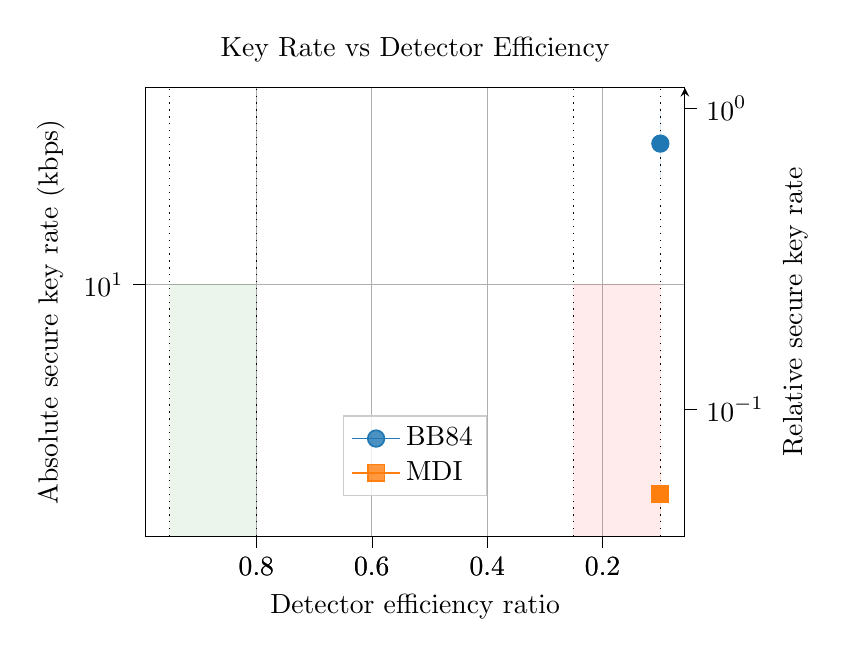
\begin{tikzpicture}

\definecolor{darkgray176}{RGB}{176,176,176}
\definecolor{darkgreen}{RGB}{0,100,0}
\definecolor{darkorange25512714}{RGB}{255,127,14}
\definecolor{darkred}{RGB}{139,0,0}
\definecolor{dimgray}{RGB}{105,105,105}
\definecolor{green}{RGB}{0,128,0}
\definecolor{lightgray204}{RGB}{204,204,204}
\definecolor{steelblue31119180}{RGB}{31,119,180}

\begin{axis}[
legend cell align={left},
legend style={
  fill opacity=0.8,
  draw opacity=1,
  text opacity=1,
  at={(0.5,0.09)},
  anchor=south,
  draw=lightgray204
},
log basis y={10},
tick align=outside,
tick pos=left,
x dir=reverse,
x grid style={darkgray176},
xlabel={Detector efficiency ratio},
xmajorgrids,
xmin=0.0575, xmax=0.9925,
xtick style={color=black},
xtick={0,0.2,0.4,0.6,0.8,1},
xticklabels={
  \(\displaystyle {0.0}\),
  \(\displaystyle {0.2}\),
  \(\displaystyle {0.4}\),
  \(\displaystyle {0.6}\),
  \(\displaystyle {0.8}\),
  \(\displaystyle {1.0}\)
},
y grid style={darkgray176},
ylabel={Absolute secure key rate (kbps)},
ymajorgrids,
ymin=1.06590488262438, ymax=57.4974902168035,
ymode=log,
ytick style={color=black},
ytick={0.1,1,10,100,1000},
yticklabels={
  \(\displaystyle {10^{-1}}\),
  \(\displaystyle {10^{0}}\),
  \(\displaystyle {10^{1}}\),
  \(\displaystyle {10^{2}}\),
  \(\displaystyle {10^{3}}\)
}
]
\path [draw=green, fill=green, opacity=0.08]
(axis cs:0.8,0)
--(axis cs:0.8,1)
--(axis cs:0.95,1)
--(axis cs:0.95,0)
--cycle;
\path [draw=red, fill=red, opacity=0.08]
(axis cs:0.1,0)
--(axis cs:0.1,1)
--(axis cs:0.25,1)
--(axis cs:0.25,0)
--cycle;
\path [draw=steelblue31119180, fill=steelblue31119180, opacity=0.15]
(axis cs:0.1,47.9650362766187)
--(axis cs:0.1,25.5858072991397)
--(axis cs:0.1,47.9650362766187)
--(axis cs:0.1,47.9650362766187)
--cycle;

\path [draw=darkorange25512714, fill=darkorange25512714, opacity=0.15]
(axis cs:0.1,1.88645556072961)
--(axis cs:0.1,1.27774021075043)
--(axis cs:0.1,1.88645556072961)
--(axis cs:0.1,1.88645556072961)
--cycle;

\addplot [semithick, steelblue31119180, mark=*, mark size=3, mark options={solid}]
table {%
0.1 35.0317595228931
};
\addlegendentry{BB84}
\addplot [semithick, darkorange25512714, mark=square*, mark size=3, mark options={solid}]
table {%
0.1 1.55254633610014
};
\addlegendentry{MDI}
\addplot [line width=0.48pt, black, dotted, forget plot]
table {%
0.8 1.06590488262438
0.8 57.4974902168035
};
\addplot [line width=0.48pt, black, dotted, forget plot]
table {%
0.95 1.06590488262438
0.95 57.4974902168035
};
\addplot [line width=0.48pt, black, dotted, forget plot]
table {%
0.1 1.06590488262438
0.1 57.4974902168035
};
\addplot [line width=0.48pt, black, dotted, forget plot]
table {%
0.25 1.06590488262438
0.25 57.4974902168035
};
\draw (axis cs:0.96122,0.01) node[
  scale=0.35,
  anchor=south east,
  text=dimgray,
  rotate=0.0
]{0.95};
\draw (axis cs:0.08878,0.01) node[
  scale=0.35,
  anchor=south west,
  text=dimgray,
  rotate=0.0
]{0.10};
\draw (axis cs:0.26122,0.01) node[
  scale=0.35,
  anchor=south east,
  text=dimgray,
  rotate=0.0
]{0.25};
\draw (axis cs:0.875,0.97) node[
  scale=0.35,
  anchor=north,
  text=darkgreen,
  rotate=0.0
]{\itshape SNSPD};
\draw (axis cs:0.175,0.97) node[
  scale=0.35,
  anchor=north,
  text=darkred,
  rotate=0.0
]{\itshape IDQ ID230 SPAD};
\end{axis}

\begin{axis}[
axis y line=right,
log basis y={10},
tick align=outside,
title={Key Rate vs Detector Efficiency},
x dir=reverse,
x grid style={darkgray176},
xmin=0.0575, xmax=0.9925,
xtick pos=left,
xtick style={color=black},
y grid style={darkgray176},
ylabel={Relative secure key rate},
ymin=0.0379237915408675, ymax=1.16861341921098,
ymode=log,
ytick pos=right,
ytick style={color=black},
ytick={0.001,0.01,0.1,1,10,100},
yticklabel style={anchor=west},
yticklabels={
  \(\displaystyle {10^{-3}}\),
  \(\displaystyle {10^{-2}}\),
  \(\displaystyle {10^{-1}}\),
  \(\displaystyle {10^{0}}\),
  \(\displaystyle {10^{1}}\),
  \(\displaystyle {10^{2}}\)
}
]
\addplot [semithick, steelblue31119180, opacity=0, mark=*, mark size=3, mark options={solid}]
table {%
0.1 1
};
\addplot [semithick, darkorange25512714, opacity=0, mark=square*, mark size=3, mark options={solid}]
table {%
0.1 0.0443182517020178
};
\end{axis}

\end{tikzpicture}
